\documentclass[12pt,a4paper,twoside]{report}
\usepackage{cs}
\usepackage{times}
\usepackage{graphicx}
\usepackage{latexsym}
\usepackage{amsmath,amsbsy}
\usepackage{amssymb}
\usepackage[matrix,arrow]{xy}
\usepackage[T1]{fontenc}
\usepackage{ae,aecompl}
\usepackage{amstext}
\usepackage{graphics}
\usepackage[T1]{fontenc}
\usepackage{ae,aecompl}
\usepackage{algorithm}
%\usepackage{algorithmic}
\usepackage{color}
\usepackage{wrapfig}
\usepackage{subcaption}
\usepackage{array}
\usepackage[table]{xcolor}
\usepackage{listings}
\usepackage{xcolor}
\usepackage{float}


\definecolor{codegreen}{rgb}{0,0.6,0}
\definecolor{codegray}{rgb}{0.5,0.5,0.5}
\definecolor{codepurple}{rgb}{0.58,0,0.82}
\definecolor{backcolour}{rgb}{0.95,0.95,0.92}

\lstdefinestyle{codestlye}{
  backgroundcolor=\color{backcolour},
  commentstyle=\color{codegreen},
  keywordstyle=\color{magenta},
  numberstyle=\tiny\color{codegray},
  stringstyle=\color{codepurple},
  basicstyle=\footnotesize,
  breakatwhitespace=false,
  breaklines=true,
  captionpos=b,
  keepspaces=true,
  numbers=left,
  numbersep=5pt,
  showspaces=false,
  showstringspaces=false,
  showtabs=false,
  tabsize=2
}

% \mastersthesis
\diplomathesis
% \leftchapter
\centerchapter
% \rightchapter
\singlespace
% \oneandhalfspace
% \doublespace

\renewcommand{\thesisauthor}{Peter Tibor ZAVACZKI}    %% Your name.
\renewcommand{\thesismonth}{June}     %% Your month of graduation.
\renewcommand{\thesisyear}{2019}      %% Your year of graduation.
\renewcommand{\thesistitle}{FINANCIAL EFFICIENCY BOOSTING SYSTEM FOR CONSUMER-GRADE PRODUCTS}
\renewcommand{\thesissupervisor}{Assoc. Prof. Dr. Eng. Delia Alexandrina MITREA}
\newcommand{\department}{\bf FACULTY OF AUTOMATION AND COMPUTER SCIENCE\\
COMPUTER SCIENCE DEPARTMENT}
\newcommand{\thesis}{LICENSE THESIS}
\newcommand{\utcnlogo}{
\includegraphics[width=15cm]{img/tucn.jpg}}

\newcommand{\uline}[1]{\rule[0pt]{#1}{0.4pt}}
%\renewcommand{\thesisdedication}{P\u{a}rin\c{t}ilor mei}

\begin{document}
%\frontmatter
%\pagestyle{headings}

\newenvironment{definition}[1][Defini\c{t}ie.]{\begin{trivlist}
    \item[\hskip \labelsep {\bfseries #1}]}{\end{trivlist}}



%\thesistitle                    %% Generate the title page.
%\authordeclarationpage                %% Generate the declaration page.

\setcounter{secnumdepth}{3}

\pagenumbering{Roman}
\setcounter{page}{1}

\begin{center}
  \utcnlogo

  \department

  \vspace{4cm}

  {\bf \thesistitle} %LICENSE THESIS TITLE}

  \vspace{1.5cm}

  \thesis

  \vspace{5.75cm}

  Graduate: {\bf \thesisauthor}

  Supervisor: {\bf \thesissupervisor}

  \vspace{3cm}
  {\bf \thesisyear}
\end{center}

\thispagestyle{empty}
\newpage

\begin{center}
  \utcnlogo

  \department

\end{center}
\vspace{0.5cm}

%\begin{small}
\begin{tabular}{p{7cm}p{8cm}}
  %\hspace{-1cm}& APPROVED,\\
  \hspace{-1cm}DEAN,                             & HEAD OF DEPARTMENT,                 \\
  \hspace{-1cm}{\bf Prof. dr. eng. Liviu MICLEA} & {\bf Prof. dr. eng. Rodica POTOLEA} \\
\end{tabular}

% \vspace{2cm}
\vspace{1.6cm}

\begin{center}
  Graduate: {\bf \thesisauthor}

  % \vspace{1cm}
  \vspace{0.6cm}

  {\bf \thesistitle}
\end{center}

\vspace{1cm}

\begin{enumerate}
  \item {\bf Project proposal:} A financial efficiency boosting system for consumer-grade products based on an extension for the Google Chrome browser, webcrawling, a web platform and a RESTful web service.
  \item {\bf Project contents:} {\it (enumerate the main component parts) Presentation page, advisor's evaluation, title of chapter 1, title of chapter 2, ..., title of chapter n, bibliography, appendices.}
  \item {\bf Place of documentation:} Technical University of Cluj-Napoca, Computer Science Department
  \item {\bf Consultants:} \thesissupervisor
  \item {\bf Date of issue of the proposal:} November 1, 2016
  \item {\bf Date of  delivery:} July 8, 2019
\end{enumerate}

\vspace{1.2cm}
\hspace{6cm} Graduate: \uline{6cm}

\vspace{0.5cm}
\hspace{6cm} Supervisor: \uline{6cm}
%\end{small}

\thispagestyle{empty}


\newpage
$ $
%\begin{center}
%\utcnlogo

%\department
%\end{center}

\thispagestyle{empty}
\newpage

\begin{center}
  \utcnlogo

  \department
\end{center}

\vspace{0.5cm}

\begin{center}
  {\bf
    Declara\c{t}ie pe proprie r\u{a}spundere privind\\
    autenticitatea lucr\u{a}rii de licen\c{t}\u{a}}
\end{center}
\vspace{1cm}



Subsemnatul(a) \textbf{PETER TIBOR ZAVACZKI} legitimat(\u{a}) cu \textbf{C.I.} seria \textbf{MM} nr. \textbf{971552} CNP \textbf{1970131245031}, autorul lucr\u{a}rii \textbf{\thesistitle}
elaborat\u{a} \^{\i}n vederea sus\c{t}inerii examenului de finalizare a studiilor de licen\c{t}\u{a} la Facultatea de Automatic\u{a} \c{s}i Calculatoare, Specializarea \textbf{CALCULATOARE, ENGLEZA} din cadrul Universit\u{a}\c{t}ii Tehnice din Cluj-Napoca, sesiunea \textbf{IULIE} a anului universitar \textbf{2018-2019}, declar pe proprie r\u{a}spundere, c\u{a} aceast\u{a} lucrare este rezultatul propriei activit\u{a}\c{t}i intelectuale, pe baza cercet\u{a}rilor mele \c{s}i pe baza informa\c{t}iilor ob\c{t}inute din surse care au fost citate, \^{\i}n textul lucr\u{a}rii \c{s}i \^{\i}n bibliografie.

Declar, c\u{a} aceast\u{a} lucrare nu con\c{t}ine por\c{t}iuni plagiate, iar sursele bibliografice au fost folosite cu
respectarea legisla\c{t}iei rom\^{a}ne \c{s}i a conven\c{t}iilor interna\c{t}ionale privind drepturile de autor.

Declar, de asemenea, c\u{a} aceast\u{a} lucrare nu a mai fost prezentat\u{a} \^{\i}n fa\c{t}a unei alte comisii de examen de licen\c{t}\u{a}.

\^{I}n cazul constat\u{a}rii ulterioare a unor declara\c{t}ii false, voi suporta sanc\c{t}iunile administrative, respectiv, \emph{anularea examenului de licen\c{t}\u{a}}.

\vspace{1.5cm}

Data \hspace{8cm} Nume, Prenume

\vspace{0.5cm}

\uline{3cm} \hspace{5cm} \textbf{\thesisauthor}

\vspace{0.5cm}
\hspace{9.4cm}Semn\u{a}tura

\thispagestyle{empty}

\newpage

\tableofcontents
\newpage

\pagenumbering{arabic}
\setcounter{page}{1}


\chapter{Introduction - Project Context}
\pagestyle{headings}

The information age has greatly revolutionalized the lives of people all around the globe, bringing along changes that made lives easier, but also more difficult at the same time. The Internet has transformed modern society into homebodies, people who do anything from the comfort of their homes rather than stepping outdoors to complete tasks. People can do it all online : shopping, chatting, paying bills, working, learning, entertaining themselves, even ordering food. Even though life is much simpler than 50 years ago, an average person probably doesn't even know of 50\% of the wonders that the World Wide Web offers them, let alone take advantage of it. That said, an increasing number of individuals use the internet every day to purchase what they need, focusing on the average Joe, who open their browser wishing to buy an item, which, in today's world can be an electronic, articles of clothing, or even groceries.

According to a statistic on the number of e-customers published in 2018 \cite{global_buyers_2017}, there were 1.66 billion individuals engaging in Business-to-Consumer e-commerce (the graph can be seen on figure \ref{fig:global_buyers_2017}), which, considering an approximate 7.55 billion population count of 2017, this would mean that 21.98\% of the global population bought something at least once in 2017 . A statistic on the frequency of purchases made by online shoppers \cite{global_frequency_2018} states that, 20\% of e-customers did online shopping once a week, 25\% once every 2 weeks, 31\% once a month, 15\% 3 to 4 times every 3 months and 10\% once every 3 months . All these 1.66 billion people, making an average of 2 purchases every month generated 2.3 trillion US dollars of revenue in 2017 and the total revenue generated by e-commerce transactions is predicted to hit 4.9 trillion US dollars by 2021, based on a statistic regarding ecommerce revenue \cite{global_revenue_2017}. This graph can be seen on figure \ref{fig:global_revenue_2017}

\begin{figure}[ht]
  \centering
  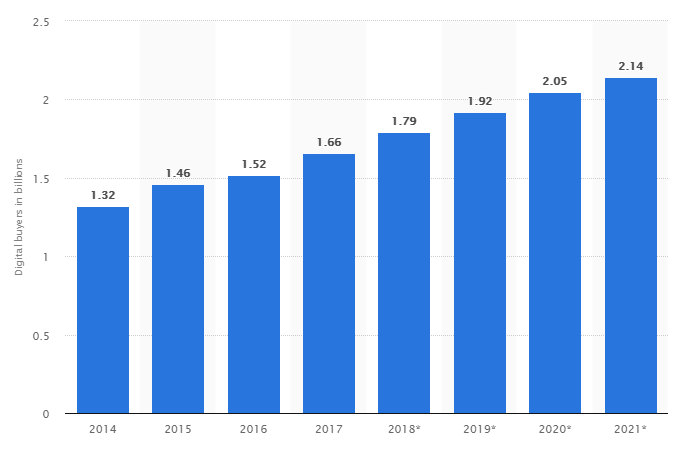
\includegraphics[width=\linewidth]{img/global_buyers_2017.png}
  \caption[]{The total number of digital buyers by year, in the 2014-2021 interval \footnotemark[1] \footnotemark[2]}
  \label{fig:global_buyers_2017}
\end{figure}

\footnotetext[1]{The numbers for the 2018-2021 interval are estimates based on the actual data}
\footnotetext[2]{Image from \cite{global_buyers_2017}}

\begin{figure}[ht]
  \centering
  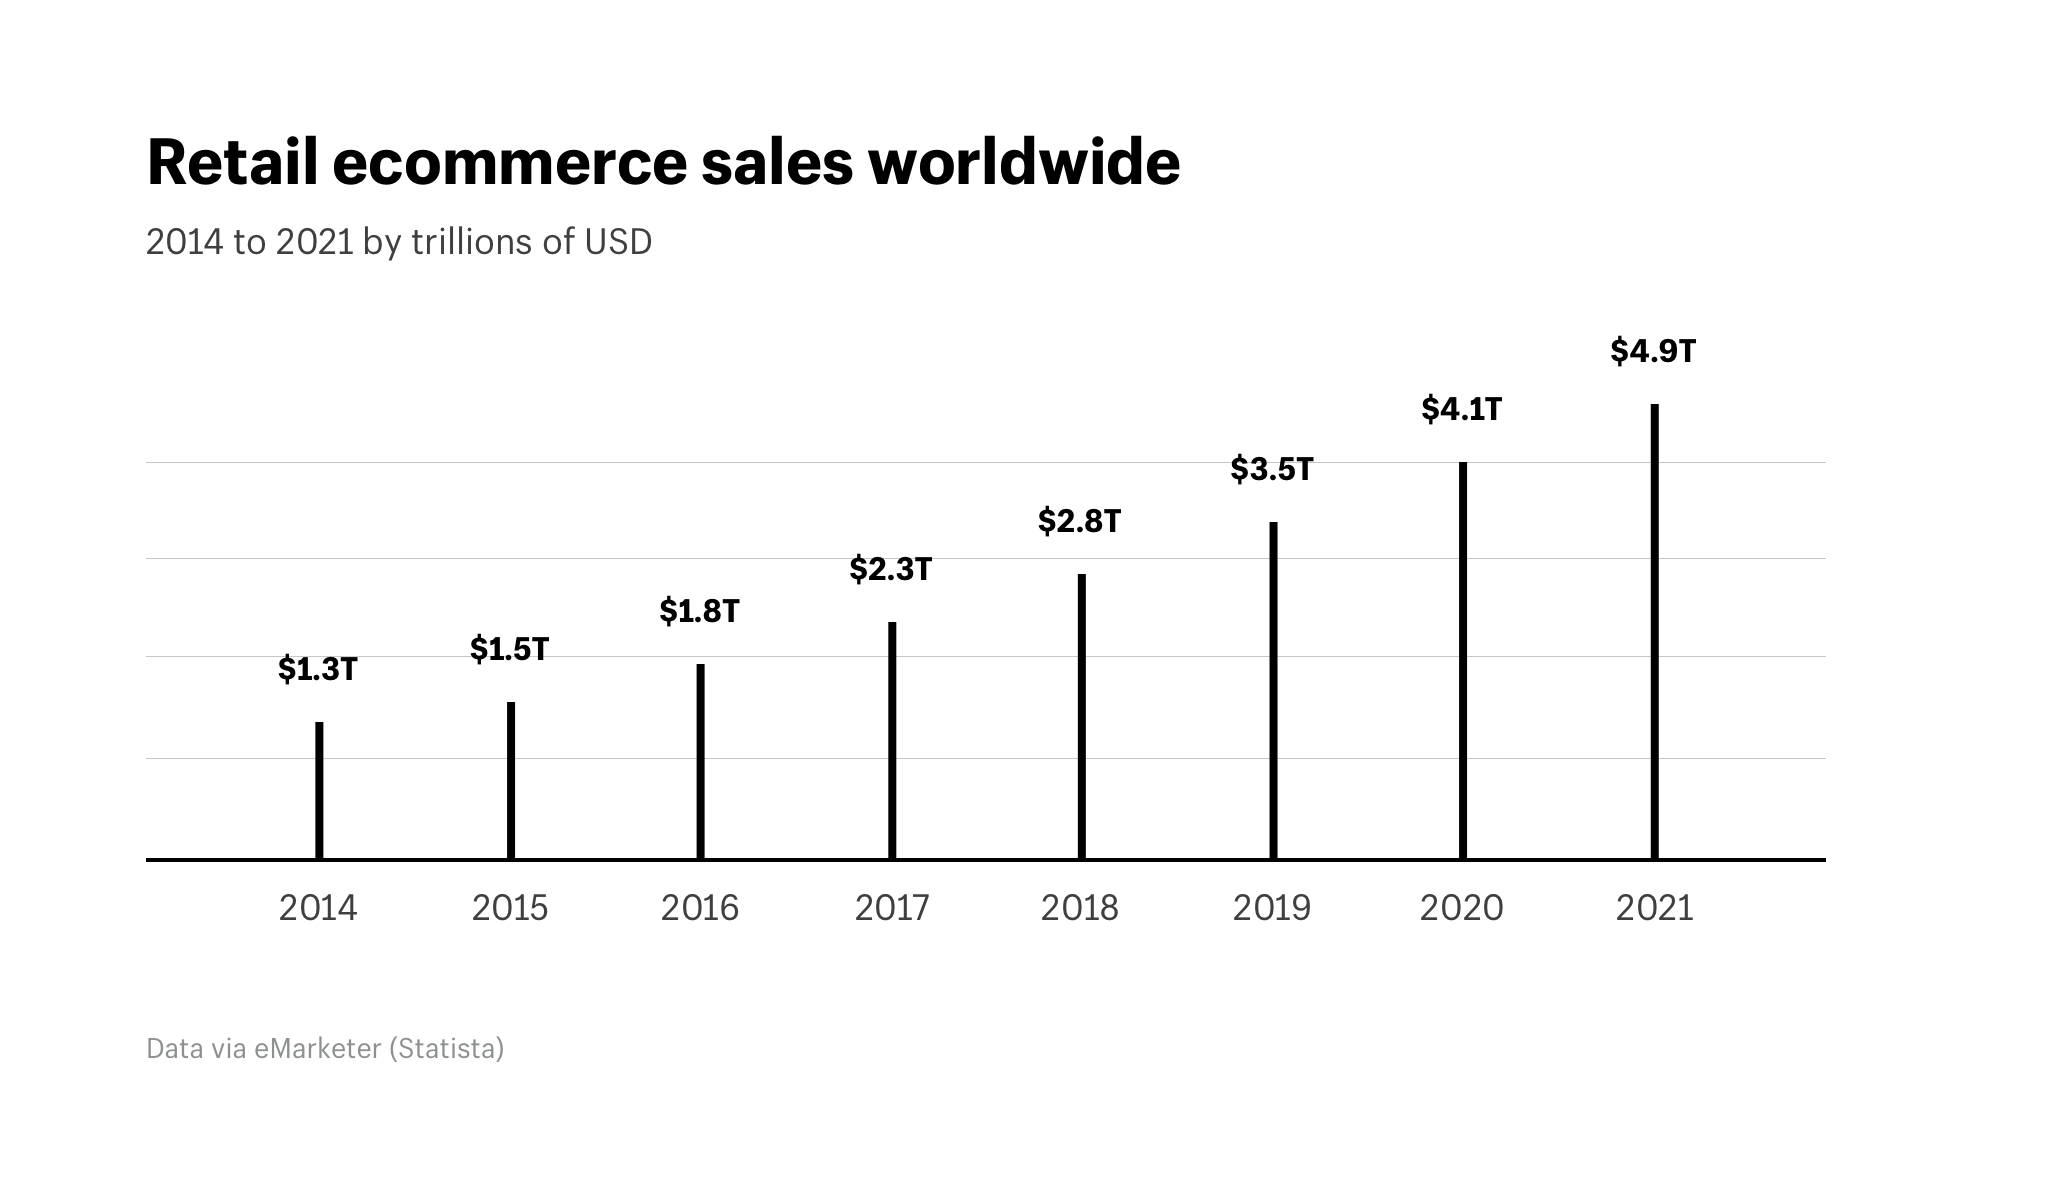
\includegraphics[width=\linewidth]{img/Retail_ecommerce_sales_worldwide.png}
  \caption[]{The total revenue generated by ecommerce sales by year, in the 2014-2021 interval \footnotemark[3]}
  \label{fig:global_revenue_2017}
\end{figure}

\footnotetext[3]{Image from \cite{global_revenue_2017_image}}

Humans as consumers, on the other side remained unchanged in two aspects which are relevant to our situation: one being that they will always try to seek the easiest way of doing a task and the other being the nature of constantly trying to spend less on the product they wish to buy. Unfortunately, from these perspectives the modern webshops can be a blessing as much as a burden. They allow you to purchase whatever you need and have it delivered to your doorstep with the minimal amound of physical work necessary. On the other hand they eliminate the option of good old bargaining, but given the vast number of retailers, prices are much more diverse also. And because of the fact that the customer can just as easily click a few times to buy a product from one retailer as from the other, the greatest way for a consumer to save money on their purchase is to find the retailer with the lowest price. As such, people who intend to save some money on their online purchases end up spending valuable amounts of time looking for a product in the webshops they know, which is a very limited number from the ocean of options they would have. These people usually end up just accepting the price they find in the first few webshops to reduce the time they spend shopping. What's more, some actually trustworthy webshops might not even have a very user-friendly interface, often confusing customers when they wish to purchase a product. This means that the probability of finding the lowest price is minimal and the process is extremely time consuming, inefficient and often tiring.

Online retailers, very similarly to their offline counterparts, have a major target in their activities too, that of reaching as many consumers as possible, and creating customers out of them. This, of course can be done via advertisements, but reaching a great amount of people with an advertisement placed on a high traffic website, such as a social network, can be extremely expensive nowadays. Taking into consideration another factor, such as the possible bad reputation the website on which the advertisement appears can also negatively impact the web retailer's or the product's image in the consumer's subconscious. The final, and probably greatest threat to the advertisement based attempts to reach customers is the usage of ad-blocking software, which modify accessed websites' DOM, completely eliminating elements containing advertisements. According to some studies regarding ad-blocking software usage \cite{adblock_stats}, 236 million desktop users actively used ad-blockig software in December 2016 and 2.3 million mobile users browsing the web from a browser that blocks advertisements by default, majorly due to the fact that 'too many ads are annoying or irrelevant'. This means that many users wont even get to see the advertisement the retailer is paying for, and even if they do, it's highly probable that it is of such poor quality or so invasive that the user will just get annoyed by it and he will develop a kind of hate for it.


\chapter{Project Objectives and Specifications}

\section{Introduction}

The purpose of this chapter is to collect, analyze, and define high-level needs and features of this license thesis. It focuses on the capabilities needed by the stakeholders and the target users, and why these needs exist.


\section{Positioning}
\subsection{Problem Statement}

Everyday more and more people are using the internet to buy what they need, from car tires to shoes, from a mobile phone to groceries. Due to the fact that the number of people shopping online increased thus increasing the demand for these opportunities, a naturally companies increased the supply by each creating one or more webshops offering the same product at different prices. This leads to the clients being lost among the options that have, and in a world where you would want to save money at every spending, a tool is necessary for the everyday webshopper to find the best price for their preferred product.

\newcolumntype{g}{>{\columncolor{lightgray}} m{0.45\linewidth}}

\begin{table}[H]
  \centering
  \begin{tabular}{| g | m{0.45\linewidth} |}
    \hline
    \textbf{The problem of}                 & looking for the cheapest offer for a product a client wishes to buy         \\
    \hline
    \textbf{affects}                        & everyday people doing their shopping online                                 \\
    \hline
    \textbf{the impact of which is}         & excessive time spent looking for an offer, ending in unsatisfactory results \\
    \hline
    \textbf{a successful solution would be} &
    easy to use
    easily accessible
    able to track the prices of a set of products across multiple webshops
    easy to extend to cover other webshops
    \\
    \hline
  \end{tabular}
  \label{table:problem_statement}
\end{table}


\subsection{Product Position Statement}

The Financial Efficiency Boosting System (FEBS) comes as a solution to the problem presented in the previous section by the use of webcrawling, a web platform and a Google Chrome extension.

\begin{table}[H]
  \centering
  \begin{tabular}{| g | m{0.45\linewidth} |}
    \hline
    \textbf{For}      & customers of webshops                                                                                           \\
    \hline
    \textbf{who}      & need a tool to simplify their search for a good price                                                           \\
    \hline
    \textbf{The FEBS} & is a system which tracks a set of products on online marketplaces                                               \\
    \hline
    \textbf{that}     & stores current data about products and tells the user about the lowest price of the product they are looking at \\
    \hline
    \textbf{unlike}   & compari.ro                                                                                                      \\
    \hline
    \textbf{The FEBS} &
    will be more accessible                                                                                                             \\
    \hline
  \end{tabular}
  \label{table:product_position_statement}
\end{table}


\section{Stakeholder and User Descriptions}
\subsection{Stakeholder Summary}

\begin{table}[H]
  \centering
  \begin{tabular}{| m{0.3\linewidth} | m{0.3\linewidth} | m{0.3\linewidth} |}
    \hline
    \rowcolor{lightgray} Name & Description                                                       & Responsibilities                                                       \\
    \hline
    \textbf{Webshop customer} & Person who engages in online shopping                             & Find the product they wish to buy and/or track                         \\
    \hline
    \textbf{Online merchant}  & Retailers of products who have their products tracked in the FEBS & Have the data about their products as clear and accessible as possible \\
    \hline
    \textbf{FEBS developer}   & Person who creates and maintains the FEBS                         & Create, improve and offer technical support for the FEBS               \\
    \hline
  \end{tabular}
  \label{table:stakeholder_summary}
\end{table}


\subsection{User Summary}

\begin{table}[H]
  \centering
  \begin{tabular}{| m{0.22\linewidth} | m{0.22\linewidth} | m{0.22\linewidth} | m{0.22\linewidth} |}
    \hline
    \rowcolor{lightgray} Name      & Description                                      & Responsibilities                                                                      & Stakeholder      \\
    \hline
    \textbf{Unregistered customer} & Person who rarely engages in online shopping     & Access the application to find a good offer                                           & Webshop customer \\
    \hline
    \textbf{Registered customer}   & Person who frequently engages in online shopping & Access the application to find a good offer and add products to their favourites list & Webshop customer \\
    \hline
  \end{tabular}
  \label{table:user_summary}
\end{table}


\subsection{User Environment}
\subsubsection{Users}

The application is public and the number of users may fluctuate based on the time of the day/week/month/year. The total number of supported users depends on the server.


\subsubsection{Time Limits}

The application should be available all the time, except for maintenance downtimes or unpredictable/uncontrollable downtimes such as power outages. A user can use the application anywhere from a minute if he finds an ideal price to a large time period if they wish to add a product to their favourites list to have it in an easily accessible location.


\subsubsection{Collaboration}

The application is used by a single person, anything a user performs with the system should not influence other users’ experience.


\subsubsection{Infrastructure}

The application will be accessible from web browsers. For full functionality a desktop based Google Chrome will be necessary, as this is the only browser to which an extension will be developed for further ease of use.


\subsection{Summary of Key Stakeholder or User Needs}

\begin{table}[H]
  \centering
  \begin{tabular}{| m{0.18\linewidth} | m{0.08\linewidth} | m{0.18\linewidth} | m{0.26\linewidth} | m{0.21\linewidth} | }
    \hline
    \rowcolor{lightgray} Need                     & Priority & Concerns             & Current solution         & Proposed solution                                        \\
    \hline
    \textbf{Support a multitude of domains}       & 0        & Customers, Merchants & Crawler for each domain  & Analyze and implement a crawler for each new domain      \\
    \hline
    \textbf{Easy to use interface}                & 1        & Customers            & Web platform             & Google Chrome extension which recognizes its environment \\
    \hline
    \textbf{Have an up to date database of items} & 1        & Customers, Merchants & Crawlers for each domain & Run the crawling task at regular intervals               \\
    \hline
  \end{tabular}
  \label{table:summary_of_key_stakeholder_or_user_needs}
\end{table}


\subsection{Alternatives and Competition}

There are similar tools currently available. One of those is compari.ro, which also lists the different webshops and prices for an item, but the fact that a client would have to actually access the website technically makes it harder to use than accessing a Google Chrome extension that is always present and provides data at one click distance.


\section{Product Overview}

The Financial Efficiency Boosting System should provide an easy to use way to users to see the best offer for their desired product. This concept can be seen in figure \ref{fig:system_diagram}.

\begin{figure}[H]
  \centering
  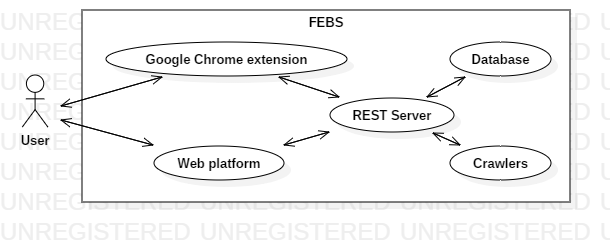
\includegraphics[width=\linewidth]{img/system_diagram.png}
  \caption{The FEBS's system diagram}
  \label{fig:system_diagram}
\end{figure}


\subsection{Product Perspective}

Compared to some competitors, such as compari.ro or PriceMon, FEBS aims to further ease the interaction of the user with the system by offering a font-end through a Google Chrome extension.
FEBS is a standalone application thus it is not part of a larger system.


\subsection{Assumptions and Dependencies}

A client is assumed to have a constant internet connection while using the application.

For the server side:

\begin{table}[H]
  \centering
  \begin{tabular}{| m{0.2\linewidth} | m{0.7\linewidth} |}
    \hline
    Database                     & \textbf{MySQL}                                                                                                              \\
    \hline
    Programming language support & \textbf{Java 8}, \textbf{Python 3}, \textbf{Angular 7}                                                                      \\
    \hline
    Frameworks, packages         & for Java: \textbf{Spring framework 2.1.3} or larger, \textbf{MySQL connector 8.0.13}, \textbf{Commons codec 1.12} or larger

    for Python: \textbf{Scrapy 1.6.0} or larger, \textbf{requests 2.22.0} or larger

    for Angular: \textbf{Angular CLI 7.2.4}                                                                                                                    \\
    \hline
    Miscellaneous                & \textbf{Node.js}, \textbf{Node Package Manager (NPM)}                                                                       \\
    \hline
  \end{tabular}
\end{table}

For the client side:

\begin{table}[H]
  \centering
  \begin{tabular}{| m{0.2\linewidth} | m{0.7\linewidth} |}
    \hline
    Web browser & \textbf{Google Chrome 75.0.3770.100} \\
    \hline
  \end{tabular}
\end{table}


\section{Product Features}

\begin{enumerate}
  \item \textbf{Simplistic web platform}

        The web platform should be as simple as possible so that the user can use and navigate it with maximum ease, while still offering the necessary features to accomplish the necessary.

  \item \textbf{Context recognition}

        The Google Chrome extension should automatically check if the user opens a link to a supported domain, in which case it automatically activates in case the user accessed the URL of a supported product it can shows different things if the webshop sells the product at the cheapest price or not: a message stating that the user is looking at the best offer or a link to the product page of the webshop with the cheapest price.

  \item \textbf{Data monitoring}

        The system tracks changes about the supported products and refreshes the already available information and each distinct running of the respective crawlers.
\end{enumerate}


\section{Other Product Requirements}

\begin{enumerate}
  \item \textbf{Visually minimalist interface}

        The front-end of the application should be as clutter-free as possible, thus improving intuitiveness and ease of use.

  \item \textbf{Usability}

        The application should require close to no input from the user, as it should recognize its working environment to automatically help the user find the cheapest offer. In case user input is necessary, it should be as intuitive as possible to do this, such as interacting with a search bar on the web platform.

  \item \textbf{Performance}

        The system’s performance is measured in the client side response time, which should be at most 5 seconds for most operations.

  \item \textbf{Availability}

        Besides maintenance downtimes, which should take at most 2 hours each week, preferably in a time period when there is as little user activity as possible, there shouldn’t be any availability issue.

  \item \textbf{Scalability}

        The application should be able to serve many concurrent users without introducing too much stress on the system.

  \item \textbf{Maintainability}

        The system should be easily maintained, as most problems could be solved by either rebooting one of the services, or fixing an outdated webcrawler.

  \item \textbf{Extensibility}

        The application should be easily extensible by adding supported products, adding URLs from supported domains to the existing products to gather data about them, or create further crawlers to support more domains.

\end{enumerate}


\chapter{Bibliographic Research}
\section{RESTful Web Services}

The concept of Representational State Transfer (REST) as an architectural style for distributed systems was invented and presented in 2000 by Roy Thomas Fielding in the 5th chapter of his doctoral dissertation \cite{fielding_rest_definition}. Fielding described it as follows: "REST provides a set of architectural constraints that, when applied as a whole, emphasizes scalability of component interactions, generality of interfaces, independent deployment of components, and intermediary components to reduce interaction latency, enforce security, and encapsulate legacy systems".

Fielding build the REST style as a hybrid style, including constraints from other, already defined architectural styles. REST was conceived from the ground up, starting with the client-server architecture, adding several constraints: statelessness, caching, a requirement for uniform interface, a layered system, and code-on-demand. The client-server architecture was used as a first step in bulding the architectural style. This was necessary in order to divide the user interface from the data storage, thus portability and scalability was improved. Adding statelessness made it mandatory that all the information necessary for the server to fulfill the request to be included in it. This means that all the information regarding the session has to be stored on the client. Statelessness is a compromise between reliability, scalability and visibility, at the downside of a potential hit in network performance due to more and more repetitive data being sent in a sequence of requests. Fortunately networking technology advanced from the, back then state of the art twisted-pair copper telephone wire solution using ADSL to provide speeds of 10 Mbit/s with 56 kbit/s download speeds being more common, while today's optic fiber solution is using the G.fast protocol to reach 1 Gbit/s speeds \cite{historical_net_speeds}, so the presented disadvantage of statelessness shouldn't be an issue nowadays. The option of caching response data was added to improve network efficiency. This means that whenever a response is sent, data should be labeled as cacheable or non-cacheable. In case a response is cacheable, a client may store and reuse the data for other equivalent requests. This allows some interactions to be eliminated, scalability and efficiency to be improved. The downside introduced with caching is that cached memory can reduce reliability due to stale data being reused. The main introduced aspect was an emphasis on making the interface between components uniform. Adding the concept of generality to the component interface simplifies the system architecture, improves the visibility of interactions and dissolves coupling between implementation and provided service, which in turn allows independent evolution of the two. The trade-off lies in decreased efficiency due to the data being passed in a standard form, rather than one tailored to the application's needs. Interface uniformization is achieved through the application of four constraints: resource identification in requests, representation based manipulation of resources, the usage of hypermedia as a means of keeping the application state and self-descriptive messages. The concept of a layered system was introduced to protect and encapsulate services, creating a downside by adding some latency to the processing of data. Finally, code-on-demand was introducted to decrease the complexity of the client.

Web services that take advantage of the REST architectural style are called RESTful web services. These kind of web services grant compatibitlity between software systems. By using RESTful web services, client systems are capable of accessing and managing web resources by using a uniform and pre-defined collection of stateless operations. Web resources are defined as documents or files identified by their Uniform Resource Identifiers (URI), and accessed using their Uniform Resource Locators (URL). RESTful web services nowadays access web resources which are exposed an a URL form. The most commonly used way to communicate with a web service is via the Hypertext Transfer Protocol (HTTP). Systems can use the URLs to send HTTP requests to the web service, which then return an HTTP response with an error message, in case something went wrong, or the data requested. The data can be the contents of a file or the result of a method called by using the web service as a Remote Method Invocation (RMI) solution, thus profiting of the code-on-demand feature or the architecture. The most common formats for representing data in an HTTP request or response is HTML, JSON or XML.


\subsection{The Spring Framework}
Spring is an application framework developed by Pivotal Software for Java, first released in 2002. It has several modules, providing a great number of services, the most important ones for me being the data access module, the inversion of control feature and the model-view-controller module.

Inversion of control (IoC) is a software engineering principle, falling into the architectual design patterns category, regarding the flow of control of the code. This principle inverts traditional flow, giving full control of execution to the used libraries, decoupling elements, increasing modularity and enabling extensibility. The concept of IoC is tightly related to the priciple of Dependency Injection. The Spring framework takes advantage of this pattern by integrating them. Dependency Injection is the standard way of linking components in the framework.

The data access module connects relational database management systems with the application using the spring framework. This is done using the Java Database Connectivity API (JDBC) and object-relational mapping tools, such as Hibernate ORM. Spring uses Hibernate ORM to map plain old java objects (POJO) to data which is supported by databases such as the MySQL relational database management system. Hibernate then further uses JDBC to connect with the database.

The most important feature of spring for my situation is the model-view-controller module, which, being a servlet and HTTP based framework, makes the creation of RESTful web services easier. The Spring MVC module is based on the architectural pattern with the same name, thus introducing the decoupling of the model, view and controller from eachother. The model part of an application is the one that deals with the object modelling of the application's domain. This term encapsulates data management and logic. As part of the model-view-controller interaction cycle, it is responsible for receiving user input from the controller, executing it and sending updates to the view if necessary. The view part of the application is an independent user interface through which information from the model is exposed to the user. The controller of the application is the part which accepts the user input, validates it if necessary and passes it to the model as commands to be executed.

The Spring framework, uniting all its modules becomes an easy to use framework that greatly helps a software developer in building web applications with the Java EE (Enterprise Edition) platform. The lowest element of a Spring MVC based application are the entities. These are the classes which model the domain of the application. The Spring framework heavily relies on a set of annotations to mark certain properties or automatically generate beans from classes which can then be injected in other classes. Entity classes are no different, as have to be marked with the '@Entity' annotation before each class definition to be discovered by the framework. The attributes of these classes have to be annotated according to the position they will fulfill in the database. Based on these annotations and the attribute names Spring can automagically generate the complete database in the defined database management system, in such a way that the created database will be a prefect representation of the application model domain, supporting the data to be manipulated. The basic communication with the database is encapsulated in interfaces called 'Repository' and annotated with the '@Service' annotation so that they can be injected in the appropriate component in the business layer. These use the objects defined as 'Entities' and execute the SQL code that Hibernate generated based on the command given to it. After executing the SQL code, JDBC gets a value or set of values from the database and returns them further into the application, to the Hibernate session, which in turn converts it to the appropriate Entity object using ORM and returns it to the calling Repository. Classes encapsulating the business logic of the application also have to be annotated with the '@Service' annotation, so that they in turn can be injected into the 'Controller' classes. The direct interfacing with the rest of the application is done via the layer of 'Controller' classes, which are annotated with the '@RestController' annotation to mark their nature, and '@RequestMapping' annotation marking the path for finding the resources that are encapsulated in it and have further annotations to aid in locating them.

Using these mechanics and architecture, Spring becomes an ideal framework to use in the creation of a RESTful web service, which would then form the back-end of a full stack application.


\section{Web scraping}

A web crawler is a bot used to automatically explore web pages on the World Wide Web as a method of web indexing. A web scraper is a specific kind of web crawler, with the difference of it being used to extract data from the visited websites. The extracted data is usually persisted in a database for later analysis and/or manipulation. Web scraping is the act of using web scrapers in a system to extract some data from websites and then persist it in a database.

A web scraper operates on a set of simple steps. First, it receives a set of URLs usually called seeds to start scraping. The scraper sends an HTTP request to the URL to fetch the page, the response usually being in the form of HTML but in case the scraper has direct access to the application API, application data can be an option, which can be encoded in JSON or other formats. The received data then has to be parsed and preferably put into objects so that it gains a uniform structure. As a final step, the processed data should be stored in a database for further use. Scrapers may have a multitude of uses, such as data mining, online price monitoring and price comparison, contact scraping, weather monitoring and website change detection.

Web scraping is a very valuable tool in the modern world, seeing as the internet is filled with so much available and useful information publicly available. The development of the internet and the amount of content it holds has been much more rapid than that of web crawling solutions. As such, the domain of web crawling is still a field with major potential and space for major breakthroughs in fields such as text processing or artificial intelligence. Web scraping solution in use nowadays include manual copying, regex matching, HTTP request based scraping, HTML parsing, DOM parsing or computer vision based web scraping. The technique of manual copying involves a human agent manually opening a website on a browser, locating the necessary data on the webpage, copying it and then pasting it into a database. This method is extremely time and money consuming, as a bot does not need to perform physical actions and does not ask for a monthly salary. Unfortunately there are some cases where automated scrapers aren't able to do the job due to scraping blockers or lack of accuracy, therefore human labor becomes necessary. The regex matching technique involves taking the whole webpage in textual form and applying a regular expression based search on it to find the data necessary. This, again is quite inefficient and might even result in inaccuracies, because website htmls can be quite lengthy, finding the correct regular expression might take a very long time, and even be so long that it's would not be worth doing. HTTP request based scraping involves directly sending HTTP requests to a public API of the website we wish to crawl, thus having its resources exposed. This is by far the most efficient scraping method, as there is not too much hassle for the development team, as they don't have to bother with parsing the website in any way. Unfortunately there aren't too many websites freely exposing their API. HTML and DOM parsing are quite similar to eachother, because in the case of HTML parsing, the code is first converted into a DOM, and from there the technique is the same: the adequate elements are selected from it to narrow down the amount of text that has to be processed by other means. HTML parsing is the most commonly used attempt to web scraping. Computer vision based web scraping is a method which appeared as a response to the attempts to block other types of scraping bots on certain sites. Computer vision brings a more modern approach to scraping by combining machine learning with image processing to locate and extract data from a website. This web scraping method is much more computationally intensive than any other one before, therefore it cannot be used as a main approach to scraping.

There are several tools that could help in web scraping or pre-build webscrapers that already solve the problem. Some of them are: cURL, 

\subsection{Scrapy}
\subsubsection{Spiders}
\subsubsection{Items and Item Pipelines}


\section{Google Chrome Extensions}

\section{Web development}
\subsection{Angular 7}



\chapter{Analysis and Theoretical Foundation}

\section{Conceptual Architecture}


\chapter{Detailed Design and Implementation}



\chapter{Testing and Validation}



\chapter{User's Manual}



\chapter{Conclusions}



%\addcontentsline {toc}{chapter}{Bibliography}
\bibliographystyle{IEEEtran}
\bibliography{thesis}%same file name as for .bib

\appendix
\chapter{Relevant code}


\chapter{Other relevant information (demonstrations, etc.)}


\chapter{Published papers}

\end{document}
